% Document Type Management
    \documentclass{book}
    \usepackage[utf8]{inputenc}
    \usepackage[english]{babel}
     
 
%  Packages for Bibiography Management
    \usepackage{biblatex}
    \usepackage{csquotes}
    \addbibresource{references.bib}


% AMS Packages
    \usepackage{amsfonts}
    \usepackage{amssymb}
    \usepackage{amsmath}
    \usepackage{amsthm}
    \usepackage{esvect}
    \usepackage{blindtext}


% Images Management Packages
    \usepackage{graphicx}
    \usepackage{epstopdf}
    \graphicspath{ {images/} }


% Packages for Tables Management
    \usepackage{booktabs}
    \usepackage{multirow}
    \usepackage{multicol}
    \usepackage{array}
    
% New Commands for text alignment within Tables    
    \newcolumntype{L}[1]{>{\raggedright\let\newline\\\arraybackslash\hspace{0pt}}m{#1}}
    \newcolumntype{C}[1]{>{\centering\let\newline\\\arraybackslash\hspace{0pt}}m{#1}}
    \newcolumntype{R}[1]{>{\raggedleft\let\newline\\\arraybackslash\hspace{0pt}}m{#1}}

% Packages to Draw Images
    \usepackage{float}
    \usepackage{tikz}
    \usetikzlibrary{shapes,backgrounds}
    \usetikzlibrary{positioning}



% Custom Section Labels   
        \newtheorem{theorem}{Theorem}[section]
        \newtheorem{conjecture}[theorem]{Conjecture}
        \newtheorem{corollary}{Corollary}[theorem]
        \newtheorem{lemma}[theorem]{Lemma}

    \theoremstyle{definition}
        \newtheorem{definition}{Definition}[section]
        \newtheorem{example}{Example}[definition]
        \newtheorem{entry}{Entry}[definition]
 
    \theoremstyle{remark}
        \newtheorem{remark}{Remark}

% Working Environment
    \newenvironment{working}{\textit{Workings. }}


% Custom Chapters and Sections
    \usepackage[explicit]{titlesec}
    
    \usepackage[many]{tcolorbox}
    \tcbset{colback=green!10!white}
    \tcbsetforeverylayer{colframe=green!10!white}
    
    \usepackage{fancyhdr}
    \usepackage{lmodern}
    \usepackage{lipsum}
    
    \definecolor{titlebgdark}{RGB}{0,163,243}
    \definecolor{titlebglight}{RGB}{191,233,251}
    
    \newlength{\chaptertopspacing}
    \setlength{\chaptertopspacing}{130pt}
    
    
    \titleformat{\chapter}[display]
      {\normalfont\huge\bfseries}
      {}
      {-\chaptertopspacing}
      {%
        \begin{tcolorbox}[
          enhanced,
          colback=titlebgdark,
          boxrule=0.25cm,
          colframe=titlebglight,
          arc=0pt,
          outer arc=0pt,
          leftrule=0pt,
          rightrule=0pt,
          fontupper=\color{white}\sffamily\bfseries\huge,
          enlarge left by=-1in-\hoffset-\oddsidemargin, 
          enlarge right by=-\paperwidth+1in+\hoffset+\oddsidemargin+\textwidth,
          width=\paperwidth, 
          left=1in+\hoffset+\oddsidemargin, 
          right=\paperwidth-1in-\hoffset-\oddsidemargin-\textwidth,
          top=0.6cm, 
          bottom=0.6cm,
          overlay={
            \node[
              fill=titlebgdark,
              draw=titlebglight,
              line width=0.15cm,
              inner sep=0pt,
              text width=1.7cm,
              minimum height=1.7cm,
              align=center,
              font=\color{white}\sffamily\bfseries\fontsize{30}{36}\selectfont
            ] 
            (chapname)
            at ([xshift=-4cm]frame.north east)
            {\thechapter};
            \node[font=\small,anchor=south,inner sep=2pt] at (chapname.north)
            {\MakeUppercase\chaptertitlename};  
          } 
        ]
        #1
        \end{tcolorbox}%
      }
    \titleformat{name=\chapter,numberless}[display]
      {\normalfont\huge\bfseries}
      {}
      {-\chaptertopspacing}
      {%
        \begin{tcolorbox}[
          enhanced,
          colback=titlebgdark,
          boxrule=0.25cm,
          colframe=titlebglight,
          arc=0pt,
          outer arc=0pt,
          remember as=title,
          leftrule=0pt,
          rightrule=0pt,
          fontupper=\color{white}\sffamily\bfseries\huge,
          enlarge left by=-1in-\hoffset-\oddsidemargin, 
          enlarge right by=-\paperwidth+1in+\hoffset+\oddsidemargin+\textwidth,
          width=\paperwidth, 
          left=1in+\hoffset+\oddsidemargin, 
          right=\paperwidth-1in-\hoffset-\oddsidemargin-\textwidth,
          top=0.6cm, 
          bottom=0.6cm, 
        ]
        #1
        \end{tcolorbox}%
      }
    \titlespacing*{\chapter}
      {0pt}{0pt}{40pt}
    \makeatother


% Custom Commands '
    \newcommand{\bb}[1]{\mathbb{#1}}
    \newcommand{\cc}[1]{\mathcal{#1}}
    \newcommand{\ovec}{\big \langle}
    \newcommand{\cvec}{\big \rangle}
    \newcommand{\m}{\cdot}


% \binomialb macro from https://tex.stackexchange.com/a/161863/4686
% expandably computes binomial coefficients with \numexpr

\begin{comment}    
    % START OF CODE
        \catcode`_ 11
        
        \def\binomialb #1#2{\romannumeral0\expandafter
            \binomialb_a\the\numexpr #1\expandafter.\the\numexpr #2.}
        
        \def\binomialb_a #1.#2.{\expandafter\binomialb_b\the\numexpr #1-#2.#2.}
        
        \def\binomialb_b #1.#2.{\ifnum #1<#2 \expandafter\binomialb_ca
                                    \else   \expandafter\binomialb_cb
                                    \fi {#1}{#2}}
        
        \def\binomialb_ca #1{\ifnum#1=0 \expandafter \binomialb_one\else 
                            \expandafter \binomialb_d\fi {#1}}
        
        \def\binomialb_cb #1#2{\ifnum #2=0 \expandafter\binomialb_one\else
                              \expandafter\binomialb_d\fi {#2}{#1}}
        
        \def\binomialb_one #1#2{ 1}
        
        \def\binomialb_d #1#2{\expandafter\binomialb_e \the\numexpr #2+1.#1!}
        
        % n-k+1.k! -> u=n-k+2.v=2.w=n-k+1.k!
        \def\binomialb_e #1.{\expandafter\binomialb_f \the\numexpr #1+1.2.#1.}
        
        % u.v.w.k!
        \def\binomialb_f #1.#2.#3.#4!%
        {\ifnum #2>#4 \binomialb_end\fi
         \expandafter\binomialb_f
         \the\numexpr #1+1\expandafter.%
         \the\numexpr #2+1\expandafter.%
         \the\numexpr #1*#3/#2.#4!}
        
        \def\binomialb_end #1*#2/#3!{\fi\space #2}
        \catcode`_ 8
    % END OR \binomialb code
\end{comment}

% ----------------------------------------------------------------------------------------------------------------------

\begin{document}

\begin{titlepage}
    \begin{center}
        \vspace*{1cm}
        
        \textbf{MATHEMATICAL PROOF STRUCTURES}
        
        \vspace{0.5cm}
        Module 4: Derivatives Pricing Theory
        
        \vspace{1.5cm}
        
        \textbf{Vernon V. Lallman}
        
        \vfill
        
        A thesis presented for the degree of Mathematics\\
        Doctor of Philosophy
        
        \vspace{0.8cm}
        
        
\includegraphics[width=0.4\textwidth]{university}
        
        Mathematics Department\\
        State University of New York \\
        Geneseo\\
        \date{\today}
        
    \end{center}
\end{titlepage}

\tableofcontents

\newpage
\chapter{PRINCIPLES OF OPTIONS PRICING}
\section{Introduction to Options Markets}
    \subsection{Derivative Markets and Instruments}
        \begin{definition}{\textbf{Derivatives}}
        These are financial instruments whose returns are derived from those of other financial instruments. Derivatives serves a valuable purpose in providing a means of managing financial risk. By using derivatives, counter parties can transfer, for a price, any undesired risk to other parties who either have risks that offset ir want to assume that risk
        \end{definition}
        
        The main types of derivative contracts are: Options, Forward Contracts, Futures Contracts, and Swaps and hybrid derivatives
        
        \begin{definition} {\textbf{Options Contracts}}
            
            An Option is a contract between two parties - a buyer and a seller - that gives the buyer the right, but not the obligation, to purchase or sell something at a later date at a price agreeded upon today. 
            
            The Option buyer pays the seller a sum of money called the \textbf{premium}. The option seller stands ready to sell or buy according to the contract terms if and when the buyer so desired. An option to buy some thing is called a \textbf{call}; an option to sell something is called a \textbf{put}.
            \end{definition}
            
            \begin{definition}{\textbf{Forward Contracts}}
            A \textbf{forward contract} is a contract between two parties - a buyer and a seller - to purchase or sell something at a later date at a price aggreed upon today.
        \end{definition}
        
        \begin{definition} {\textbf{Futures Contracts}}
            
            A futures contract is also a contract between two parties - a buyer and a seller - to but or sell something at a future date at a price agreed upon today. Futures contracts evolved out of forwards contracts and posses many of the same characteristics. Unlike forward contracts, futures contracts trade on organized exchanges.  
            
            The buyer of a futures contract, who has the obligation to buy the good at a later date, can sell the contract in the futures market, which relieves her of the obligation to purchase the good. Otherwise the seller of a contract, who is obligated to sell the good at the later date, can buy the contract back in the futures market, relieving him of the obligation to sell the good.  
            
            
            \textbf{Options on futures}, somtimes called \texttt{commodity options} or \texttt{futures options}, are an important synthesis of futures and options markets. An opiton on futures contract gives the buyer the right to buy or sell a futures contract at a later date at a price agreed upon today. 
        \end{definition}
        
        \begin{definition}{\textbf{Swaps and hybrid Derivatives}}
            
            A swap is a contract which two parties agree to exchange cash flows. For example, one party is currently receiving cash from one investment but would prefer another type of investment in whcih the cash flows are different. The party contact a swap dealer, a firm operating in the over-the-counter market, who takes the opposite side of the transaction. The firm and the dealer, in effect, swap cash flow streams. Depending on what happens to prices or interest rates , one party might elect to tie the payments it makes on the swap contract to the price of a commodity, called a \textbf{swaption}.
            
            Some of these types of contracts are referred to as \textbf{hybrid derivatives} because they combine the elements of several other types of contracts. 
        \end{definition}
        
        \begin{tcolorbox}[colback=blue!5!white,colframe=blue!75!black, title=Sticky Note]
            The Different types of derivatives include options, forwards, futures, options on futures, swaps, and hybrids.
        \end{tcolorbox}
    
    \newpage 
    \subsection{Important Concepts in Financial and Derivative Markets}
        
        \begin{definition}{\textbf{Market Efficiency and Theoretical Fair Value}}
            
            Market Efficiency is a characteristic of a market in which the prices of the instruments trading therein reflect their true economic value to investors. In an efficient marketplace, prices fluctuate randomly and investors cannot consistently earn returns above those that would compensate them for the level of risk they assume.
            
            An efficient market is one in which the price of an asset equals its true economic value, which is called the \textbf{theoretical fair value}. Spot and derivative markets are normally quite efficient. 
        \end{definition}
        
        \begin{tcolorbox}[colback=blue!5!white,colframe=blue!75!black, title=Sticky Note]
            An efficient market is one in which the price of an asset equals its true economic value, which is called the theoretical fair value. Spot and derivative markets are normally quite efficient
        \end{tcolorbox}        
        
        \begin{definition}{\textbf{Repurchase Agreements}}
            
            A repurchase agreement (known as \textbf{repos} is a legal contract between a buyer and a seller; the seller agree to sell currently a specific asset to the buyer - as well as buy it back (usually) at a specified time in the future ar an agreeed upon price. 
            
            Derivatives traders often need to be able to borrow and lend money in the most effective manner possible. Repos are often very low-cost way of borrowing money, 
        \end{definition}
        
        \begin{definition}{\textbf{Risk \& Return}}
        
            Return is the numerical measure of investment performance. They are two main meassure of return:
                \begin{itemize}
                    \item \textbf{Dollar Return} measures investment performance as total dollar profit or loss
                    
                    \item \textbf{Percentage Return} measures investment performance per dollar invested
                \end{itemize}
            
            Risk is uncertainty about future returns. The return investors expects is composed of the risk-free rate and a risk premium. This relationship is illustrated in Figure \ref{fig:1RiskReturn}, where $E(r_s)$ is the expected return on the spot asset, $r$ is the risk-free rate, and $E(\phi)$ is the risk premium - the excess of expected return over the risk-free rate.
               
                \begin{figure}[h]
                    \centering
                        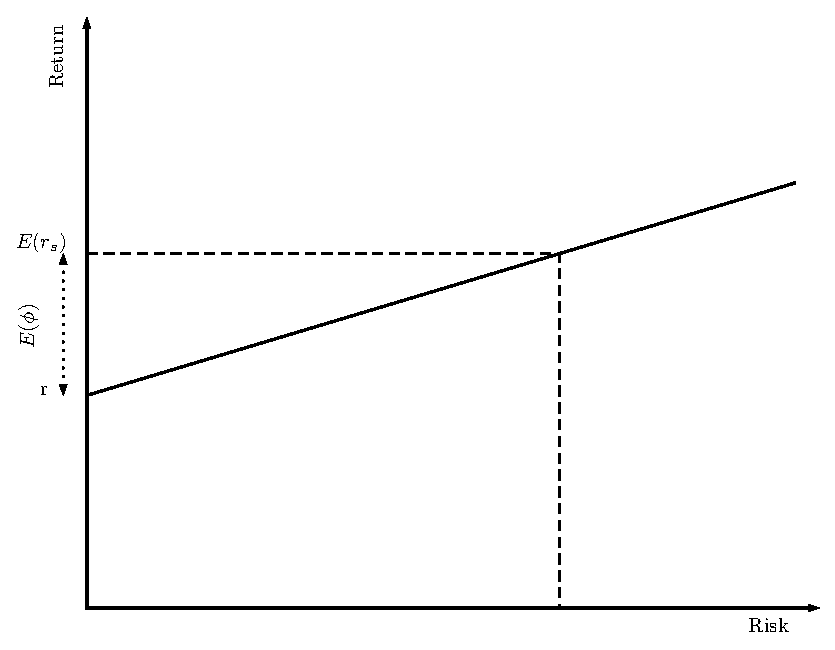
\includegraphics[scale=0.65]{images/fig:1RiskReturn.eps}
                    \caption{Risk-Return Trade-Off}
                    \label{fig:1RiskReturn}                
                \end{figure}
            
            Note the direct relationship between risk and expected return; this relationship is known as \textbf{risk-return tradeoff}. This trade-off arises because all investors seek ti maximizze expected returns subject to to minimal level of risk. 
            
        \end{definition}
        
        
        \begin{definition}{Risk and Return and Arbitrage}
            
            Expected Return is the return one expects to earn. A portion of the expected return must compensate for the \textit{opportunity cost}, as represented by the risk-free rate. The excess of the expected return over the risk-free rate is called the \textbf{risk premium}. In general, we say that 
                \begin{equation}
                    E(r_s)= r + E(\phi)
                \end{equation}
            where $E(r_s)$ is the expected return from some investment identified as "$s$", "$r$" is the risk-free rate, and $E(f)$ is expected risk premium. By the Capital Asset Pricing Model (CAPM), the expected risk premium can be articulated more clearly as: 
                \begin{equation}
                    E(r_s) = r + [E(r_m)]\beta_s
                \end{equation}
            where $E(r_m)$ is the expected return on the market portfolio, which is the combination of all risky assets, and $b_s$ is called the asset's beta. The \textbf{beta} is a measure of the risk that an investor cannot avoid, which is the risk that the asset contributes to the porfolio. The CAPM assumes that individual diversify away as much risk as possible amd hold the market portfolio. Thus, the only risk that matters is the risk that a given asset contributes to a diversfed portfolio.
            
            We use derivatives to reduce or eliminate the risk out of a portfolio. with risk out of the picture, all one really needs to understand is arbitrage. \textbf{Arbitrage} is a condition resulting from the fact that two identical combination of assets are selling for different prices. An investor who spots such an opportunity will buy the lower-priced combination and sell the higher priced combination. Becuase the combination of assets perform identically, the performance of one combination hedges the performance of the other so that the risk is eliminated. 
        \end{definition}
    
    \newpage
    \subsection{Fundamental Linkages between Spot and Derivative Markets}
        \begin{definition}{Arbitrage \& Law of One Price}
            
            \textbf{Arbitrage} is a type of transaction in which an investor seek to profit when the same good sells for two different prices. The individual engages in arbitrage, called the arbitrageur, buys the good at the lower price and immediately sells it at the higher price. The lower price will be drived up and the high price driven down until the two prices are equal. 
            
            \textbf{The law of one price} requires that equivalent combinatiron of assets, meaning those that offer the same outcome, must sell for a single price or else there would be an opportunity for porfitable arbitrage that woulld quickly eliminate the price differential. Markets ruled by the Law of one price have the following four characteristics: 
                \begin{enumerate}
                    \item Investors always prefer more wealth to less
                    \item Given two investments opportunities, investors will prefer one that performs at least as well as the other in all states and better in at least one state
                    \item If two investment opportunities offer equivalent outcomes, they must have equivalent prices. 
                    \item An investment opportunity that produces the same return in all states is risk-free abd nust earn the risk-free rate. 
                \end{enumerate}
            Occasionally prices get out of line. Arbitrage is the mechanism that keeps prices in line.
        \end{definition}
        
        \begin{tcolorbox}[colback=blue!5!white,colframe=blue!75!black, title=Sticky Note]
            The law of one price requires that equivalent combinations of assets, meaning those that offer the same outcomes, must sell for a singe price or else there would be an opportunity for profitable arbitrage that would quickly elimate the price differential. 
        \end{tcolorbox}        
        
        \begin{definition}{The Storage Mechanism: Spreading Consumption across Time}
        
            Storage is an important linkage between the spot and derivatives markets. Many types of assets can be purchased and stored. Holding a stock or bond is a form of storage. Even making a loan is a form of storage. Storage is a form of investment in which one defers selling the item today in anticupation of selling it at a later date. Storage spreads consumption across time. 
            
            Because price constantly fluctuate, storage entails tisk. Derivatives can be used to reduce the risk by providing a means of establishing today the item's future sale price. This suggests that the risk entails in storing the item can be removed. In that case, the overall investment should offer the risk-free rate. Therefore, it is not suprising that the prices of the storable item, the derivative contract, and the risk-free rate will all be related. 
        \end{definition}
    
        \begin{definition}{Delivery \& Settlement}
            At expiration, a forward or futures contract call for either immediate delivery of the item or cash payment of the same value. Thus, an expiring forward or futures contract is equivalent to the spot transaction. The price of the expiring contract, therefore, must equal the spot price. Though options differ somewhat from forwards and futures at expiration, there instruments have a n unambiguous value at expiration that is determined bt the spot price. 
        
        \end{definition}
        
    \newpage    
    \subsection{Role of the Derivatives Markets}
        \begin{definition}{\textbf{Risk Management}}
            
            Becuase derivative prices are related to the price of the underlying spot market goods, they can be used to reduce or increase the risk of owning the spot items. Hence, they are two major groups of participants in the derivative markets: 
                \begin{itemize}
                    \item \textbf{Hedgers}: participants seeking to reduce risk
                    \item \textbf{Speculators}: participants seeking to increase risk
                \end{itemize}
        \end{definition}
            Derivatives market enable hedger to transfer their unwanted risk to speculators and its enable speculators to accumulate the hedger's unwanted risk. Because the derivatives markets effective at allocating risks among investors, no one need assume an uncomfortable level of risk.
            
        \begin{definition}{\textbf{Price Discovery}}
            Futures market are considered a primary means for determining the spot price of an asset. Since, spot market is large, fragmented, and sometimes information deficient, participants rely on the futures markets to assemble the fragmented information into a type of consensus, reflecting the spot price of the particular asset on which the futures contract is based. The \textbf{nearby contract} is often treated as the spot price.
            
            Hence, futures and forwards markets are said to provide price discovery. Options markets do not directly provide forecasts of future spot prices. They fo, however, provide valuable information about the volatility and, hence, the risk of the underlying spot price. 
        \end{definition}
        
        \begin{definition}{\textbf{Operational Advantages}}
            
            Derivatives markets off several operational advantages:
                \begin{enumerate}
                    \item Low Transaction Cost attracts and engages many market participants
                    
                    \item Derivatives Markets are often more liquid than spot market
                    
                    \item Participants can customize their portfolio in accordance with their risk preference
                \end{enumerate}
        \end{definition}
        
        \begin{definition}{\textbf{Market Efficiency}}
            Derivative markets provides a means od managing risk, discovering prices, reducing costs, improving liquidity, selling short, and making the both spot and futures marketplaces more efficient
        \end{definition}
        
        \begin{tcolorbox}[colback=blue!5!white,colframe=blue!75!black, title=Sticky Note]
            Derivative markets provide a means of managing risk, discovering prices, reducing costs, imporving liquidity, selling short, and making the market more efficient. 
        \end{tcolorbox}        

\newpage
\section{Structure to Options Markets}
    \subsection{History of Options Markets}    
    \subsection{Call Options}
    \subsection{Put Options}
    \subsection{Over-the-Counter Options Market}
    \subsection{Organized Options Trading}
        \subsubsection{Listing Requirements}
        \subsubsection{Contract Size}
        \subsubsection{Exercise Prices}
        \subsubsection{Expiration Dates}
        \subsubsection{Position \& Exercise Limits}
    \subsection{Options Exchanges \& Trading Activity}
    \subsection{Options Traders}
        \subsubsection{Market Makers}
        \subsubsection{Floor Broker}
        \subsubsection{Order Book Offical (Board Broker)}
        \subsubsection{Other Option Trading Systems}
        \subsubsection{Off-Floor Options Traders}
        \subsubsection{Cost \& Profitability of Exchange Membership}
    \subsection{Mechanics of Trading}
        \subsubsection{Placing an Opening Order}
        \subsubsection{Tole of the Clearinghouse}
        \subsubsection{Placing an Offsetting Order}
        \subsubsection{Exercising an Option}
    \subsection{Option Price Quotations}
    \subsection{Types of Options}
        \subsection{Stock Options}
        \subsubsection{Index Options}
        \subsubsection{Currency Options}
        \subsubsection{Other Types of Options}
        \subsubsection{Real Options}
    \subsection{Transaction Costs in Option Trading}
        \subsubsection{Floor Trading \& Clearing Fees}
        \subsubsection{Commissions}
        \subsubsection{Bid-Ask Spread}
        \subsubsection{Other Transaction Costs}
    \subsection{Regulation of Options Markets}
    
%---------------------------------------------------------------------------------------------------------------------------
\newpage
\section{Principles of Options Pricing}

In this chapter, we do not derive the exact price of an option, rather, we confine the discussion to identifying upper and lower limits and factors that influence an option's price. In later chapters we will explain how the exact options price is determined.  
   
    \subsection{Basic Notation \& Terminology}
        The following are the symbols used thoughout this module:
            \begin{itemize}
                \item $S_0 =$ stock price today (time 0 = today)
                \item $X =$ exercise price
                \item $T =$ time to expiration as defined below
                \item $r =$ risk-free rate as defined below
                \item $S_T =$ stock price at option's expiration, that is after the passage of a time of $T$
                \item $C(S_o, T, X) =$ price of a call option in which the stock price is $S_0$, the time to expiration is $T$, and the exercise price is $X$
                \item $P(S_o, T, X) =$ price of a call option in which the stock price is $S_0$, the time to expiration is $T$, and the exercise price is $X$
            \end{itemize}
        In some situations, we need to distinguish an American Call from a European Call. If so, the call price will be denoted as either $C_a(S_o, T, X)$ or $C_e(S_o, T, X)$ for the American and European Calls, respectively. If there is no $a$ or $e$ subscript, the call can be either an American or European Call. In the case where two options differ only by exerise price, the notations $C(S_o, T, X_1)$ and $C(S_o, T, X_2)$ will identify the prices of the calls with $X_1$ less than $X_2$, so $X_1 < X_2$. Similarly, in the case two options differ only by time to expiration, the times to expiration will be $T_1$ and $T_2$ where $T_1<T_2$. The options' prices will be $C(S_o, T_1, X)$ and $C(S_o, T_2, X)$. Identical adjustments will be made for put option prices
        
        For most of the examples, we shall assume that the stock pays no dividends. If, during the life of the option, the stock pays dividends of $D_1, D_2, ... $, and so forth, then  we can make a simple adjustment and obtain similar results. To do so, simply subtract the present value of the dividends
            \begin{equation}
                \sum_{j=1}^{N} D_j( = 1+r)^t_j
            \end{equation}
        Where $N$ is the dividends, $t_j$ is the time to each dividends day, from the stock price, and $r$ is the risk-free rate earned on a riskless investment
        
        To illustrate the principles of options pricing, we shall be using prices for options on DCRB, a fictional technology company traded on NASDAQ. These prices were assumed to be observed on May 14 and presented in table \ref{tab:montage}. DCRB is currently trading at \$125.94. The May options expire on May 21, the June options expire on June 18, and the July options expire on July 16.
        

            \begin{table}[h]
                \centering
                \caption{DCRB Option Data, May 14}
                \label{tab:montage}
                \begin{tabular}[h]{lllll}
                    \toprule
                    & & Time Value & Time Value & Time Value \\
                    Exercise Price & Intrinsic Value & May & June & July \\
                    \midrule
                    \$120.00 & \$5.94 & \$2.81 & \$9.46 & \$14.96 \\
                    \$125.00 & \$0.94 & \$4.81 & \$12.56 & \$17.66 \\
                    \$130.00 & \$5.94 & \$3.60 & \$11.35 & \$16.40 \\
                    \bottomrule
                \end{tabular}     
            \end{table}
            
        And the prevailing risk-free rates 
        
        The May options expire on May 21, the June options expire on June 18, and the July options expire on July 16. Table \ref{tab:DCRBRiskTime} illustrates the prevailing risk-free rates and calculated time to expiration. 
        
                \begin{table}[h]
                        \centering
                        \caption{The Prevailing Risk-Free Rates and Time to Expiration of DCRB Options}
                        \label{tab:DCRBRiskTime}
                        \begin{tabular}[h]{L{1.5cm} L{1cm} L{1cm} L{1cm} }
                        \toprule
                            & May & June & July  \\
                         \midrule
                            4.57\%  & 4.56\%    & 4.65\% \\
                            0.0192  & 0.0959    & 0.1726 \\
                        \bottomrule
                        \end{tabular}
                \end{table}          
    
    \newpage
    \subsection{Principles of Call Option Pricing}
        \subsubsection{Minimum Value of a Call}
            A call option is an instrument with limited liability. If the call holder see that it is advantageous to exercise it, the call will be exercised. If exercising it will decrease the call holder's wealth, the holder will not exercise it. The call options cannot have negative value, becuase the holder cannot be forced to exercise it. Therefore, 
                \begin{equation}
                    C(S_0, T, X) \geqq 0
                \end{equation}
            For an American Call, the statement that a call option has a minimum value of zero is dominated by a much stronger statement: 
                \begin{equation}
                    C_a(S_0, T, X) \geqq Max(, S_0 - X)
                \end{equation}
            
        \begin{tcolorbox}[colback=blue!5!white,colframe=blue!75!black, title=Sticky Note]
            Because a call option need not be exercised, its minimum value is zero 
        \end{tcolorbox}              
            
            The minimum value of an option is called its \textbf{intrinsic value}, sometimes referred to as \textbf{parity value}, \textbf{parity}, or \textbf{exercise value}. Intrinsic value, which is positive for in-the-money calls and zero for out-of-the-money calls, is the value the call holder receives from exercising the option and the value the call writer gives up when the option is exercised. 
            
        \begin{tcolorbox}[colback=blue!5!white,colframe=blue!75!black, title=Sticky Note]
            The intrinsic value of an American call is the greater of zero or the difference between the stock price and the exercise price. 
        \end{tcolorbox}              
            
            To prove that $C_a(S_0, T, X) \geqq Max(, S_0 - X)$, consider the DCRN June \$120.00 call. The current price of the stock is $\$125.94$, and the exercise price is \S120.00. Evaluating the expression gives:
                \begin{align*}
                    C_a(S_0, T, X) & \geqq Max(0, S_0 - X) \\ 
                    C_a(\$125.94, 35, \$120.00) & \geqq Max(0, 125.94-120.00) \\
                    C_a(\$125.94, 35, \$120.00) & \geqq \$5.94
                \end{align*}
            Now, consider the following scenarios: 
                \begin{enumerate}
                    \item \textbf{Call Price $<$ Intrinsic Price}
                        If the call were priced at less than \$5.94 --say, \S3.00. An option trader could buy the call for \$3.00, exercise it - which would entail purchasing the stock for \$120.00 and then sell the stock for \$125.94. This arbitrage transaction would net an immediate riskless profit of \$2.94 per share. Arbitrageur exploiting this riskless opportunity would push the mispriced call option price back to at least \$5.94. Thus, \$5.94 is the minimum price of the call.
                                
                    \item \textbf{Exercise Price $>$ Stock Price}
                        If the exercise price exceeds the stock price, as do the options with an exercise price of $\$130.00$. Then $Max(0, \$125.94 - \$130.00) = \$0.00$, and the minimum value will be zero. 
                \end{enumerate}
        
            
            Now look at all of DCRB calls. Those with an exercise price of $\$120.00$ have a minimum value of $Max(0, \$125.94 - \$120.00) = \$5.94 $. All three calls with an exercise price of $\$120.00$ have a minimum have prices no less than $\$5.94$. The calls with an exercise price of $\$125.00$ have a minimum value of $max(0, \$125.94 -\$125.00) = \$0.94$ and are priced at no less than $\$0.94$. The calls with an exercise price of $\$130.00$ have minimum values of $Max(0, \$125.94 - \$130.00) = 0$. All those options with strike prices below $\$125.94$ obviously have nonnegative values. Thus, all the DCRB call options conform quite closely to the rule. 
            
            The price of an American call normally exceeds its intrinsic value. The difference between the call price and its intrinsic value is called the \textbf{Time Value} or \textbf{Speculative Value} of the call, which is defined as $C_a(S_0, T, X) - Max(0, S_0 -X)$. Time value reflects what tradres are willing to pay for the uncertainty of the underlying stock.
                
                \begin{table}[h]
                    \centering
                    \caption{Intrinsic Value and Time Values of DCRB Calls}
                    \label{tab:callTime}
                    \begin{tabular}[h]{L{1.5cm} L{1.5cm} | L{1cm} L{1cm} | L{1cm} L{1cm} | L{1cm} L{1cm} }
                    \toprule
                        \multicolumn{2}{c}{} & \multicolumn{2}{c}{May} & \multicolumn{2}{c}{June} & \multicolumn{2}{c}{July} \\\cline{3-8}
                        Exercise Price & Intrinsic Value  & Time Value & Call Price & Time Value & Call Price & Time Value & Call Price \\
                    \midrule
                        120.00 & 5.94 & 2.81 & 8.75 & 9.46 & 15.40 & 14.96 & 20.90 \\
                        125.00 & 0.94 & 4.81 & 5.75 & 12.56 & 13.50 & 17.66 & 18.60 \\    
                        130.00 & 0.00 & 3.60 & 3.60 & 11.35 & 11.35 & 16.40 & 16.40 \\
                    \bottomrule
                    \end{tabular}
                \end{table}                
                
            Table $\ref{tab:callTime}$ presents the intrinsic values and time values of DCRB Calls. note that the time value increases with the time to expiration.
            
                \begin{figure}[H]
                    \centering
                        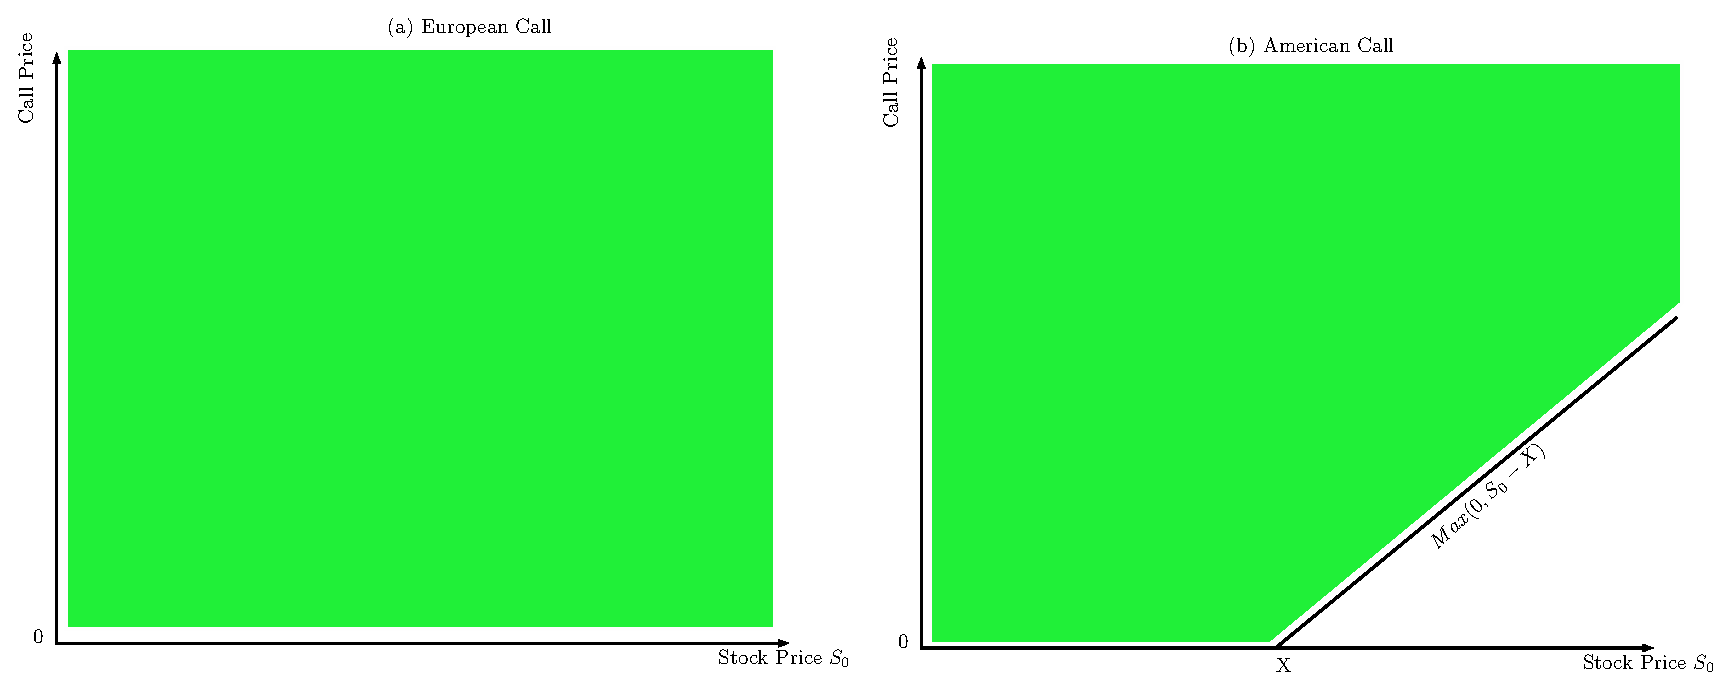
\includegraphics[scale=0.45]{images/fig:CallMin.eps}
                    \caption{Minimum Values of European \& American Calls}
                    \label{fig:2CallMin}                
                \end{figure}
            
            Figure \ref{fig:2CallMin} illustrates what we have already established so far. The call price in the shaded area. Figure \ref{fig:2CallMin} (a) illustrates the European call price can lie in the entire area. This does not mean that the American call price is less than the European call price but only that is range of possible values is narrower.
            
        \begin{tcolorbox}[colback=blue!5!white,colframe=blue!75!black, title=Sticky Note]
            The time value of an American call is the difference bwtween the call price and the intrinsic value
        \end{tcolorbox}              
            
        \subsubsection{Maximum Value of a Call}
            A call option has a maximum value: 
                \begin{equation}
                    C(S_0, T, X) \leqq S_0
                \end{equation}
        
        \begin{tcolorbox}[colback=blue!5!white,colframe=blue!75!black, title=Sticky Note]
            The maximum value of a call is the price of the stock. 
        \end{tcolorbox}  
            
            The maximum value of a call is the price of the stock. However, one call that asympotically approaches worth of the underlying stock must maturity that asympotetic approaches infinity.
            
            Figure $\ref{fig:CallMinMax}$ adds the maximum value rule to Figure \ref{fig:2CallMin}. Notice that the maximum value property has significantly reduced the possible option values. 
            
                \begin{figure}[h]
                    \centering
                        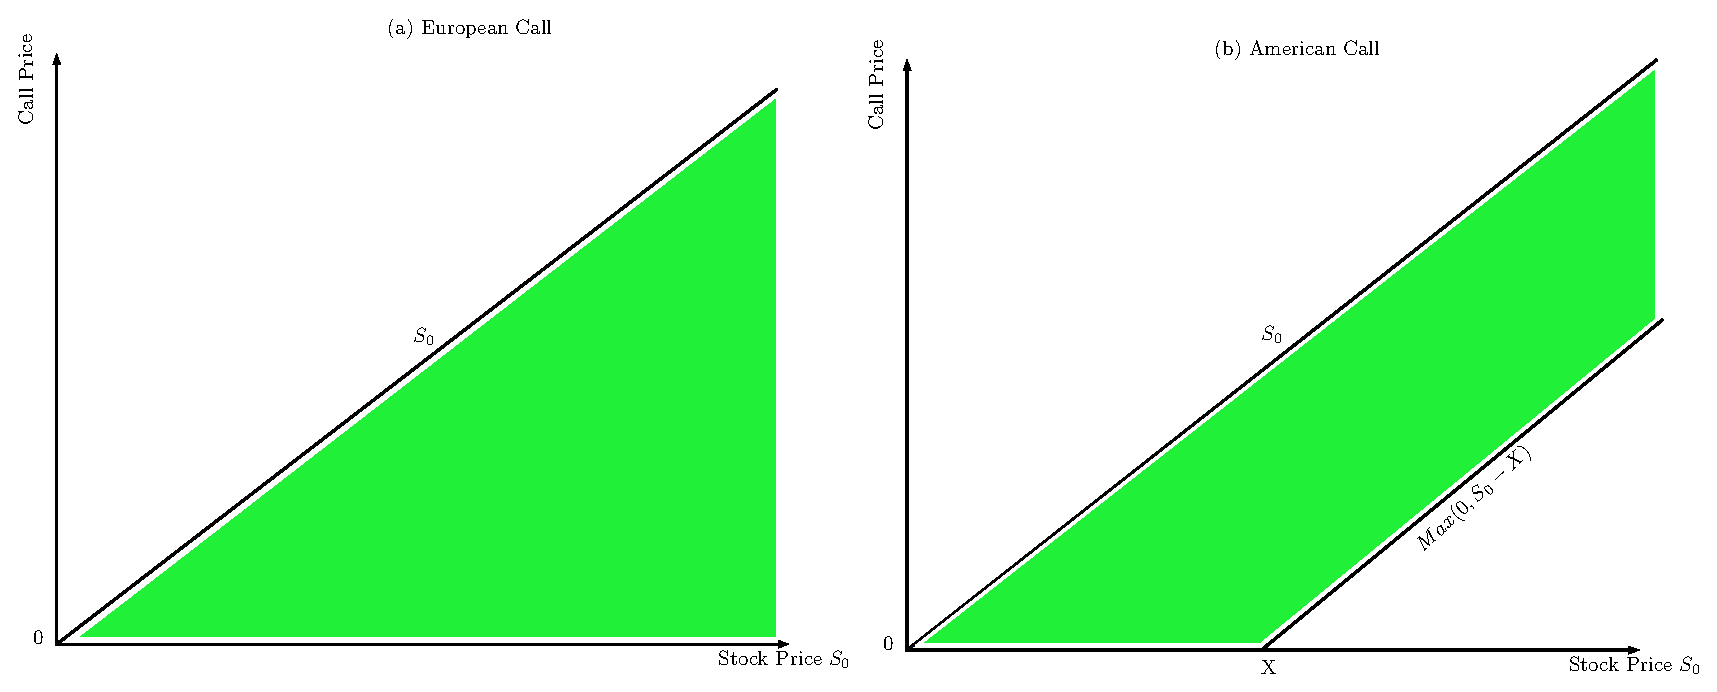
\includegraphics[scale=0.45]{images/fig:CallMinMax.eps}
                    \caption{Minimum \& Maximum Values of European \& American Calls}
                    \label{fig:CallMinMax}                
                \end{figure}
            
        \subsubsection{Value of a Call at Expiration}
            The price of a call option at expiration is given as:
                \begin{equation}
                    C(S_T, O, X) = Max(0, S_T - X)
                \end{equation}
            At expiration, a call option is worth the intrinsic value becuase no time remains in the option's life. This rule holds for both American and European options.
            
                \begin{figure}[h]
                    \centering
                        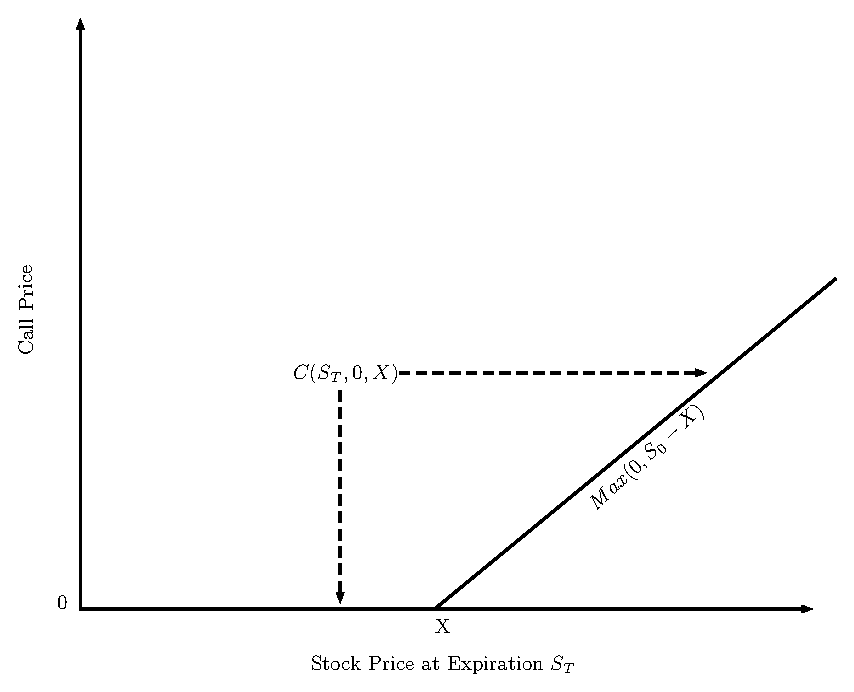
\includegraphics[scale=0.65]{images/fig:CallExp.eps}
                    \caption{The Value of a Call at Expiration}
                    \label{fig:CallExp}                
                \end{figure}            
            Figure $\ref{fig:CallExp}$ illustrates the value of a call at expiration. This is one situation in which the value of the call is unambiguous. But do not confuse this with our ultimate objective, which is to find the value of the call prior to expiration.
   
        \subsubsection{Effect of Time to Expiration}
            Consider two American call options wtih price of $C_a(S_0,T_1,X)$ and $C_a(S_0,T_2,X)$, respectively, where $T_2 > T_1$. Two answer the question: which option have the greater value. 
            
            Suppose that today is the expiration date of the short-lived option, then the value of option is $$ C_a(S_0,T_1,X) = C_a(S_0, 0, X) = Max(0, S_{T_1}-X$$. The longer dated option expires in $T_2 - T_1$ and the current stock price is $S_0 = S_{T_1}$, so it's minimum value is  $C_a(S_0, T_2, X) = Max(0, S_{T_1}-X)$ Therefore $$ C_a(S_0, T_2, X) \geqq C_a(S_0, T_1, X) $$. Thus, a longer lived American call must always be worth at least as much as a shorter-lived American call with the same terms. 
            
        \begin{tcolorbox}[colback=blue!5!white,colframe=blue!75!black, title=Sticky Note]
            A longer-lived American call must at least be worth at least as much as a shorter-lived American call with the same terms. 
        \end{tcolorbox}              
            
            The time value of a call option varies with the time to expiration and the proximity  of the stock price to the exercise price. Investors pay for the time value of the call based on the uncertaintly of the future stock price. If the stock price is very high, the call is said to be \textbf{deep-in-the-money} and the time value will be low. If the stock price is very low, the call is said to be \textbf{deep-out-of-the-money} and the time value likewise will be low. The time value is low at these extremes, the probability of the call expiring in or out-of-the-money is lower. The uncertainty is greater whrn the stock price is near the exercise price, and it is at this point that time value is higher. 
            
                \begin{figure}[h]
                    \centering
                        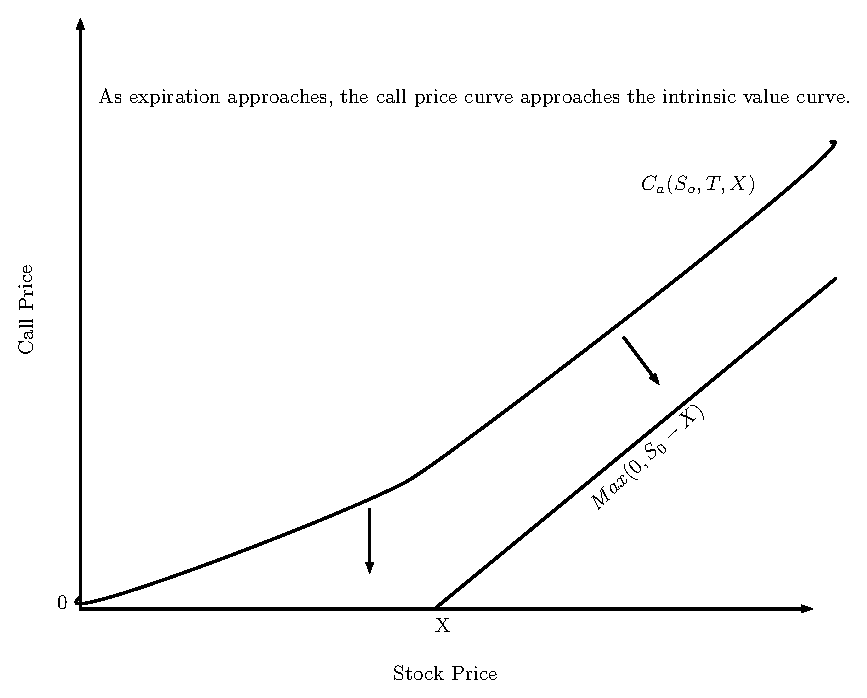
\includegraphics[scale=0.65]{images/fig:ACallExp.eps}
                    \caption{The Price Curve for American Calls}
                    \label{fig:ACallExp}                
                \end{figure}
            
            These properties of time value and our previous results enable us to get a general idea of what the call price looks like relative to the stock price. Figure \ref{fig:ACallExp} illustrates this point for American calls. The curved line is the price of the call, which lies above the intrinsic value, $Max(0, S_0 -X$. As expiration approaches, the call price loses its time value, a process called \textbf{time value decay}, and the curve moves graudally towards the intrisic value. At expiration , the call price curve collapes onto the intrinsic value and the curve looks exactly like Figure \ref{fig:CallExp}. 
        \subsubsection{Effects of Exercise Price}
            \begin{definition}{\textbf{Effect on Option Value}}
                
                Consider two European calls that are identical in all respects except that the exercise price of one is $X_1$ and the other is $X_2$, such that $X_2 > X_1$. We want to know whch price is greater $C_e(S_0, T, X_1)$ or $C_e(S_0, T, X_2)$. 
                
                Now consider two portfolios, a \textbf{money spread} portfolio and a risk-free bonds portfolio. Portfolio A consists of a long position in the call with the exercise price of $X_1$ and a short position in the call with the exercise price of $X_2$. Because we pay $C_e(S_0, T, X_1)$ and received $C_e(S_0, T, X_2)$, this postion will have an initial value of $C_e(S_0, T, X_1) - C_e(S_0, T, X_2)$. 
                
                Portfolio B consists simply of risk-free bonds with a face value of $X_2 - X_1$. These bonds should be considered as a pure discount instruments, like treasury bills, and as maturing at the opiton's expiration. Thus, the value of this portfolio is the present value of the bonds' face value $$ (X_2 - X_1)(1+r)^{-T} $$.
                
                Firstly, let's determine the value of portfolio A at expiration. The value of the portfolio is contingent on the portfolio cash flow or payoff when the options expires and the stock price at expiration, $S_T$. The stock price at expiration has three possible ranges:
                    \begin{itemize}
                        \item $S_T \leqq X_1 < X_2$
                        \item $X_1 < S_T < X_2$
                        \item $X_1 < X_2 \leqq S_T$
                    \end{itemize}
                
                Table \ref{tab:moneyspread} illustrates the values of the portfolios A and B at expiration. Portfolio A reaches it's maximal profit when underlying security is above $X_2$ at expiration, its maximal loss when the stock price falls below $X_1$. Also the portfolio breakevens when stock price is hovering at level calculate by adding the spread difference to the portfolio's lower strike, $X_1$.  
                
                \begin{table}[h]
                    \centering
                    \caption{The Effect of Exercise Price on Call Value: Payoff at Expiration of Portfolios A \& B}
                    \label{tab:moneyspread}
                        \begin{center} 
                        \begin{tabular}[h]{lll}
                        \toprule
                            Stock Price v. Exercise Price & Profit/Loss \& Breakeven & Description \\
                        \midrule    
                            $S_T \leqq X_1 < X_2$ & $0 - C_e(S_0, T, X_1) - C_e(S_0, T, X_2)$ & Maximum Loss\\
                            $X_1 < S_T < X_2$ & $S_T - K_1 - C_e(S_0, T, X_1) - C_e(S_0, T, X_2)$ & Direct Relationship \\
                            $X_1 < S_T < X_2$ & $X_1 + C_e(S_0, T, X_1) - C_e(S_0, T, X_2)$ & Breakeven \\
                            $X_1 < X_2 \leqq S_T$ & $X_2 - X_1 - C_e(S_0, T, X_1) - C_e(S_0, T, X_2)$ & Maximum Profit \\
                            $(X_2 - X_1)(1+r)^{-T}$ & $X_2 - X_1 > 0$ & Riskless \\
                        \bottomrule
                        \end{tabular} 
                        \end{center}
                \end{table}                
                
                Because the portfolio receives a payoff of $S_T -X_2$, when the long call leg expires in-the-money and the written call has a payoff of $-S_T + X_2$. Adding the payoffs from the two options shows that the portfolio A will always produce a payoff of no less than zero and, in some cases, more than zero. Therefore, $$ C_e(S_0, T, X_1) \geqq C_e(S_0, T, X_2) $$. We have proven this result only for European calls. With American calls the long call need not be exercised, so we need only consider what would happen if the short call were exercised early. 
                
                Suppose that the stock price prior to expiration is $S_t$ and exceeds $X_2$. For whatever reason, the out-of-the-money short call is exercised. This produces negative cash flow, $-(S_t - X_2)$. The protfolio manager then exercises the long call, which produces a positive cash flow of $S_t - X_1$. The sum of these two cash flows is $X_2 - X_1$, which is positive because $X_2$ is strictly greater than $X_1$. Thus, early exercise will not generate a negative cash flow. Portfolio A therefore will never produce a negative cash flow at expiration, even if the options are American Calls. Hence, our result holds for both American and European Calls $$ C(S_0, T, X_1) \geqq C(S_0, T, X_2) $$. 
                
        \begin{tcolorbox}[colback=blue!5!white,colframe=blue!75!black, title=Sticky Note]
            The price of a European call must be at least as high as the price of an otherwise identical European call with a higher exercise price.
        \end{tcolorbox}  
                
                The prices of the DCRB calls adhere to the predicted relationships. The lower the exercise price, the higher the call option price.
            
        \begin{tcolorbox}[colback=blue!5!white,colframe=blue!75!black, title=Sticky Note]
            The price of an American call must be at least as high as the price of an otherwise identical American call with a higher exercise price 
        \end{tcolorbox}              
            \end{definition}
            
            \begin{definition}{\textbf{Limits on the Difference in Premiums}}
                
                Notice from Table \ref{tab:moneyspread} that portfolio's B returns is never less than portfolio A. Therefore an investor would never pay less for portfolio B than for portfolio A. The price of portfolio A is $C_e(S_0, T, X_1) - C_e(S_0, T, X_2)$, the price of the option purchased minus the price of the options sold. The price of portfolio B is $ (X_2 - X_1)(1+r)^{-T} $, the present value of the bond's face value. Thus, $$ (X_2 - X_1)(1+r)^{-T}  \geqq C_e(S_0, T, X_1) - C_e(S_0, T, X_2) $$
                
        \begin{tcolorbox}[colback=blue!5!white,colframe=blue!75!black, title=Sticky Note]
            The difference in prices of two European calls that differ only by exercise price cannot exceed the present value of the diffrence in their exercise prices 
        \end{tcolorbox}  
                
                A related and useful statement is $$ (X_2 - X_1)  \geqq C_e(S_0, T, X_1) - C_e(S_0, T, X_2) $$
                This follows because the difference in the exercise prices is greater than the present value of the difference in the exercise prices. 
                
                For American calls, the call with the lower exercise price is worth at least as much as the call with the higher exercise price. However, the statement that the difference in premiums cannot exceed the present value of the difference in exercise prices does not hold for the American call. If both calls are exercised at time $t$ before expiration and the payoff of $X_2 - X_1$ is invested in risk-free bonds, portfolio A's return will be $(X_2 - X_1)(1+r)^{T-t}$ which exceeds portfolio B's return of $X_2 - X_1$. Thus, portfolio B will not always out perform or match portfolio A.
                
                If however, the bonds purchased for portfolio B have a face value of $(X_2 - X_1)(1 + r)^T$, and thus a present value of $X_2 - X_1$. Thus, portfolio B will always outperform portfolio A. In that case, the current value of portfolio A cannot exceed that of portfolio B. Accordingly, we can state that for American calls, $$ (X_2 - X_1)  \geqq C_a(S_0, T, X_1) - C_a(S_0, T, X_2) $$
                
        \begin{tcolorbox}[colback=blue!5!white,colframe=blue!75!black, title=Sticky Note]
            The difference in the prices of two American calls the differ only by exercise price cannot exceed the difference in their exerrcise price
        \end{tcolorbox}                  
                
                Table \ref{tab:callExPrice} presents the approximate calculations for examining these properties on the DCRB Calls. Consider the May 120 and 125 calls. Using Table \ref{tab:callTime} and Table \ref{tab:DCRBRiskTime} we can see that that their difference in premiums is $8.75 - 5.75 = 3.00$. The present value of the difference in exercise  prices is $PV_{120, 125} = 5(1 + \frac{4.57}{100})^-0.0192 = 4.9957$. The remaining combinations are calcualted similarly using the appropirate risk-free rate and time to expiration for those options, referenced in Table \ref{tab:DCRBRiskTime}. Becuase these are American calls, the difference in their prices must be no greater than the difference in their exercise prices. As Table \ref{tab:callTime} shows, all the calls conforms to this condition. In addition, all the differences in the call prices are less than the present value of the difference between the exercise prices. Remember that this result need not hold for American calls because they can be exercised early. 

                \begin{table}[h]
                    \centering
                    \caption{The Relationship between Exercise Price \& Call Price for DCRB Puts}
                    \label{tab:callExPrice}
                    \begin{tabular}[h]{L{1.5cm} L{1.5cm} | L{1cm} L{1cm} | L{1cm} L{1cm} | L{1cm} L{1cm} }
                    \toprule
                        \multicolumn{2}{c}{} & \multicolumn{2}{c}{May} & \multicolumn{2}{c}{June} & \multicolumn{2}{c}{July} \\\cline{3-8}
                        Exercise Price & Spread Future Value & Spread Present Value & Call Spread & Spread Present Value & Call Spread & Spread Present Value & Call Spread \\
                     \midrule
                        120, 125 & 5    & 4.9957    & 3.00  & 4.9787    & 1.90  & 4.9611    & 2.30 \\
                        120, 130 & 10   & 9.9914    & 5.15  & 9.9573    & 4.05  & 9.9222    & 4.50 \\
                        125, 130 & 5    & 4.9957    & 2.15  & 4.9787    & 2.15  & 4.9611    & 2.20 \\
                    \bottomrule
                    \end{tabular}
                \end{table}              
            
            \end{definition}
            
            
        \subsubsection{Lower Bound of a European Call}
        
            Consider two portfolios, A and B. Portfolio A consists of  a single share of long stock currently priced at $S_0$, while portfolio B contains a long European call priced at $C_e(S_0,T, X$ and risk-free bonds with a face value of X and, therefore, a present value of $X(1+r)^{-T}$. The current value of portfolio B is thus $$ C_e(S_0, T, X) + X(1+r)^{-T} $$

                \begin{table}[h]
                    \centering
                    \caption{The Lower Bound of an European Call: Payoffs at Expiration of Portfolio A \& B}
                    \label{tab:EcallLB}
                        \begin{center} 
                        \begin{tabular}[h]{llll}
                        \toprule    
                            Portfolio & Current Value & $S_T \leqq X$ & $S_T > X$ \\
                        \midrule    
                            A & $S_0$ & $S_T$ & $S_T$ \\
                            B & $C_e(S_0, T, X) + X(1+r)^{-T}$ & X & $(S_T - X) + X = S_T$ \\
                        \bottomrule
                        \end{tabular} 
                        \end{center}
                \end{table}            
            
            The payoffs from these two portfolios are shown in Table \ref{tab:EcallLB}. The return on portfolio B is always at least as large as the returns on portfolio A and sometimes larger. Investors will recognize this fact and price portfolio B at a value at least as great as portfolio A's; that is $$ C_e(S_0, T, X) + X(1+r)^{-T} \geqq S_0 $$. Rearranging this expression yields $$ C_e(S_0, T, X) \geqq S_0 - X(1+r)^{-T} $$
            If $ S_0 - X(1+r)^{-T} < 0$, we invoke the rule that the minimum value of a call is zero. Combining these results gives us a lower bound of
                \begin{equation}
                     C_e(S_0, T, X) = Max \left[ 0, S_0 - X(1+r)^{-T} \right]
                \end{equation}

        \begin{tcolorbox}[colback=blue!5!white,colframe=blue!75!black, title=Sticky Note]
            The price of an European call must at least equal the greater of zero or the stock minus the present value of the exercise price.
        \end{tcolorbox} 
            
            If the European call price is less than the stock price minus the present value of the exercise price, we canm construct an arbitrage portfolio. We buy the call and risk-free bonds and sell short the stock. This portfolio has a positive initial cash flow, because the call price plus the bond price is less than the stock price. At expiration, the payoff is $X - S_T$ if $X > S_T$ and zero otherwise. The portfolio has a positive cash value today and either zero or positive cash flow at expiration. Again no way to lose money. 
            
                \begin{figure}[h]
                    \centering
                        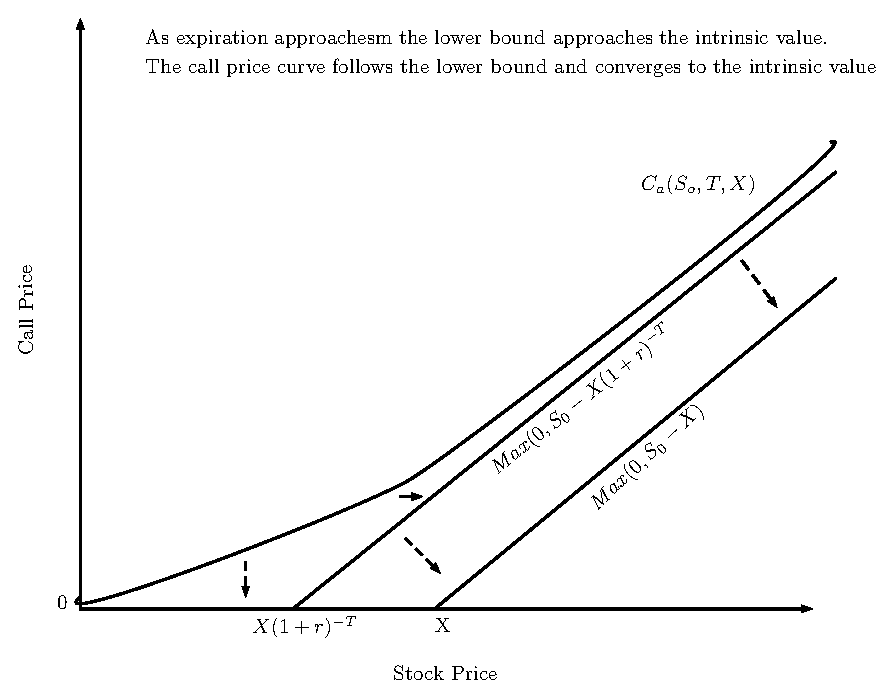
\includegraphics[scale=0.65]{images/fig:ECallExp.eps}
                    \caption{The Price Curve fo European Calls}
                    \label{fig:ECallExp}                
                \end{figure}
            
            Figure \ref{fig:ECallExp} shows this result for European calls. The curved line is the call price, which must lie above the lower bound. As expiration approaches, the time to expiration decreases such that the lower bound moves to the right. The time value decreases on the option as well and follows the lower bound, with all eventually converging to the intrinsic value, $Max(0, S_0 - X$, at expiration. 
            
            Consider two European call that differ by their times to expiration, $T_1$ and $T_2$. Their prices are $C_e(S_0, T_1, X)$ and $C_e(S_0, T_2, X))$, respectively. At time $T_1$, the shorter-lived option expires and is worth $Max(0, S_{T_1} - X$. The minimum value of the longer-lived option is $Max(0, S_{T_1} - X)(1+r)^{-(T_2 - T_1)}$. Thus, the value of the short-lived option is less than the lower bound of the long lived option. Therefore, the longer-lived call must be priced at least as high as the shorter-lived call. 

        \begin{tcolorbox}[colback=blue!5!white,colframe=blue!75!black, title=Sticky Note]
            The European calls, a longer-lived call will always be worth at least as much as a shorter-lived call with the same terms. 
        \end{tcolorbox} 
    
            Consider two European calls that  differ by the time to expiration, $T_1$ and $T_2$. Their prices are $C_e(S_0, T_1, X)$ and $C_e(S_0, T_2,X)$, respectively. At time $T_1$ the shorter-lived option expires and is worth $Max(0, S_{T_1} - X)$. The minimum value of the longer-lived option is $Max\left( 0, S_{T_1} - X(1+r)^{-(T_2 - T_1)} \right)$. Thus, the value of the longer-lived option is less tahn the lower-bound of the longer-lived option. Therefore, the longer-lived call must be priced at least as high as the shorter-lived call. 
            
            We should note that if the stick pays dividends such that the stock price minus the present value of the dividends is $S'_0 = S_0 - \sum_{j=1}^N \left [ D_j (1 + r)^{-t_j} \right]$, then the lower bound is restated as 
               
                \begin{equation}
                    C_e(S_0, T, X) = Max
                         \begin{cases}
                            0 \\
                            S_0 - \sum_{j=1}^N \left [ D_j (1 + r)^{-t_j} \right] - X(1+r)^{-T} \\
                        \end{cases}
                \end{equation}
                
            Suppose that instead of options on stocks, the option is on a foreign currency. The exchange rate is represented by $S_0$, but we must recognize that the currency pays interest at the discrete compounding rate of $\rho$. This is the foreign riskfree rate, which is obtained in the same manner we did for treasury bills. If we buy  oone unit of currency, it will grow to $(1 + \rho)^T$ units at time $T$.
            
            Let us redefine portfolio A to consists of $(1+ \rho)^{-T}$ units of currency. Becuase of the accumulation of interest, the $(1 + \rho)^{-T}$ units of currency will grows to $(1+ \rho)^{-T}(1+ \rho)^{T} = 1$ untis of currency. Then, the payoffs are the same at the orginal portfolio. The only difference in this case is that the initial  value of portfolio A is now defined as $S_0(1+ \rho)^{-T}$. The lower bound of the Foreign currency European call then becomes

                \begin{equation}
                    C_e(s_0,T,X) \geqq Max
                         \begin{cases}
                            0 \\
                            S_0(1+ \rho)^{-T} - X(1 + r)^{-T} \\
                        \end{cases}
                \end{equation}
            
        \subsubsection{Early Exercise of American Calls on Dividend-Paying Stocks}
            When a company declares a dividend, it specifies that the dividend is payable to all stock holders as of a certain date, called the \textbf{holder-of-record} date. Two business days before the holder-of-record date is the \textbf{ex-dividend} date. To be a stock holder of record by the holder-of-record date, one must buy the stock by the ex-dividend date. The stock price tends to fall by the amount of the dividend on the ex-dividend date. 
            
            When a stock goes ex-dividend, the call price drops along with it. The amount by which the call price falls cannot be determined at this point in our understanding of options pricing. Since the call is a means of obtaining the stock, however, its price could never change by more than the stock price change. Thus, the call price will fall by no more than the dividend. An investor could avoid this loss in value by exercising the options immediately before the stock goes ex-dividend. This is the only time the call should be exercised early
            
        \begin{tcolorbox}[colback=blue!5!white,colframe=blue!75!black, title=Sticky Note]
            It may be optimal to exercise an American call early if the stock is about to go ex-dividend.
        \end{tcolorbox}             
        
            Another way to see that early exercise occur is to recall that we stated that the lower bound of a European call on a dividend paying stock is 
        
                \begin{equation*}
                    C_e(S_0, T, X) = Max
                         \begin{cases}
                            0 \\
                            S_0 - \sum_{j=1}^N \left [ D_j (1 + r)^{-t_j} \right] - X(1+r)^{-T} \\
                        \end{cases}
                \end{equation*}
                
            To keep things simple assume, assume only one dividend of the amount D, and that the stock will go ex-dividend in the next instant. Then, the stock price adjusted for dividends, $S'_0 \approx S_o - D$ (since the present value of D is almost D). Since we would consider exercising only in-the-money calls assume that $S_0 > X$. By exercising the option, the call holder obtains the value $S_0 - X$.
            
            Suppose that you were holding a European call whose value was only slightly above the lower bound. Then you might wish it were an American call because an American call could be exercised to capture the value $S_0 - X$. If you were holding a European call and wished it were an American call foe at least that instant,  then it should be obvious that the right tp early exercise would have value. So an American call could be worth more than a European call. The value of the right to exercise early is what distinguishes an American call from a European call. The right is only worth something when there is a dividend on the stock. Am similar argument applies when the underlying is a currency, which pay interest. 
        
        \subsubsection{Effect of Interest Rates}
        
            Interest rate affects a call in several ways:
                \begin{itemize}
                    \item Interest rates affect the lower bound of call prices. The lower the interest rate, the lower the lower bound. In the extreme case case of a zero interest rate, the lower bound would be the same as the intrinsic value. Nothing happens to the option price if the interest rate is zero. 
                    \item The higher the interest rate, the more interest the investor can earn on the money saved by buying the option to purchase the stock at a later date. Thus, when interest rates increase, calls are more attractive to the buyers so they will have higher prices. 
                \end{itemize}

        \begin{tcolorbox}[colback=blue!5!white,colframe=blue!75!black, title=Sticky Note]
            The price of a call is directly related to interest rates
        \end{tcolorbox}   

        \subsubsection{Effect of Stock Volatility}
            Higher risk in a stock translates into greater value for a call option on it. This is because greater volatility increases the gains on the call if the stock price increases, because the stock price can then exceed the exercise price by a larger amount. On the other hand,  greater volatility means that if the stock goes down, it can be much lower than the exercise price. To a call holder, however, this is does not matter beucase the potential for losses is limited; it is said to be truncated at the exercise price. 
            
            Another way to understand the effect of volatility on the call price is to consider the extreme case of zero volatility. If the stock price is less than the exercise price, the absence of volatility guarantees that the option will expire out-of-the-money. No one would pay anything for this option. If the stock price exceeds the exercise price and has zero volatility, it will expire in-the-money and be worth $S_T - X$ at expiration, where $S_T$ is the future value of $S_0$. In this case, the call will then simply be a risk-free asset worth $S_0$ minus the present value of $X$. Since volatility does not affect the lower bound, the call price and lower bound remain above the intrinsic value, reflecting the fact that the option will still not be exercised until expiration. On the other hand, high volatility is what makes call options attractive, and the investors are willing to pay higher premiums on options with greater volatility. 
            
        \begin{tcolorbox}[colback=blue!5!white,colframe=blue!75!black, title=Sticky Note]
            The price of a call is directly related to the voaltility of the underlying stock. 
        \end{tcolorbox}             
            
    \subsection{Principles of Put Options Pricing}
    
        \subsubsection{Minimum value of a Put}
    
            A put is an option to sell a stock. A put holder is not obligated to exercise it and will not do so if exercising will decrease wealth. Thus, a put can never have a negative value: $P(S_0, T, X) \geqq 0$. An American put can be exercised early. Therefore, 
            
                \begin{equation}
                    P_a(S_0,T,X) \geqq Max(0, X - S_0)
                \end{equation}
            
        \begin{tcolorbox}[colback=blue!5!white,colframe=blue!75!black, title=Sticky Note]
            Becuase a put option need not be exercised, its minimum value is zero
        \end{tcolorbox}             
            
            Suppose that DCRB June 130 put sells for less than $X - S_0$. Let the put sell for $\$3.00$. Then it would be worthwile to buy the stock for $\$125.94$, buy the put for $\$3.00$, and exercise the put. This would net an immediate risk-free profit of $\$1.06$. The combined actions of all investors conducing this arbitrage would force the put price up to at least $\$4.06$, the difference between the exercise price and the stock price.
            
                \begin{figure}[h]
                    \centering
                        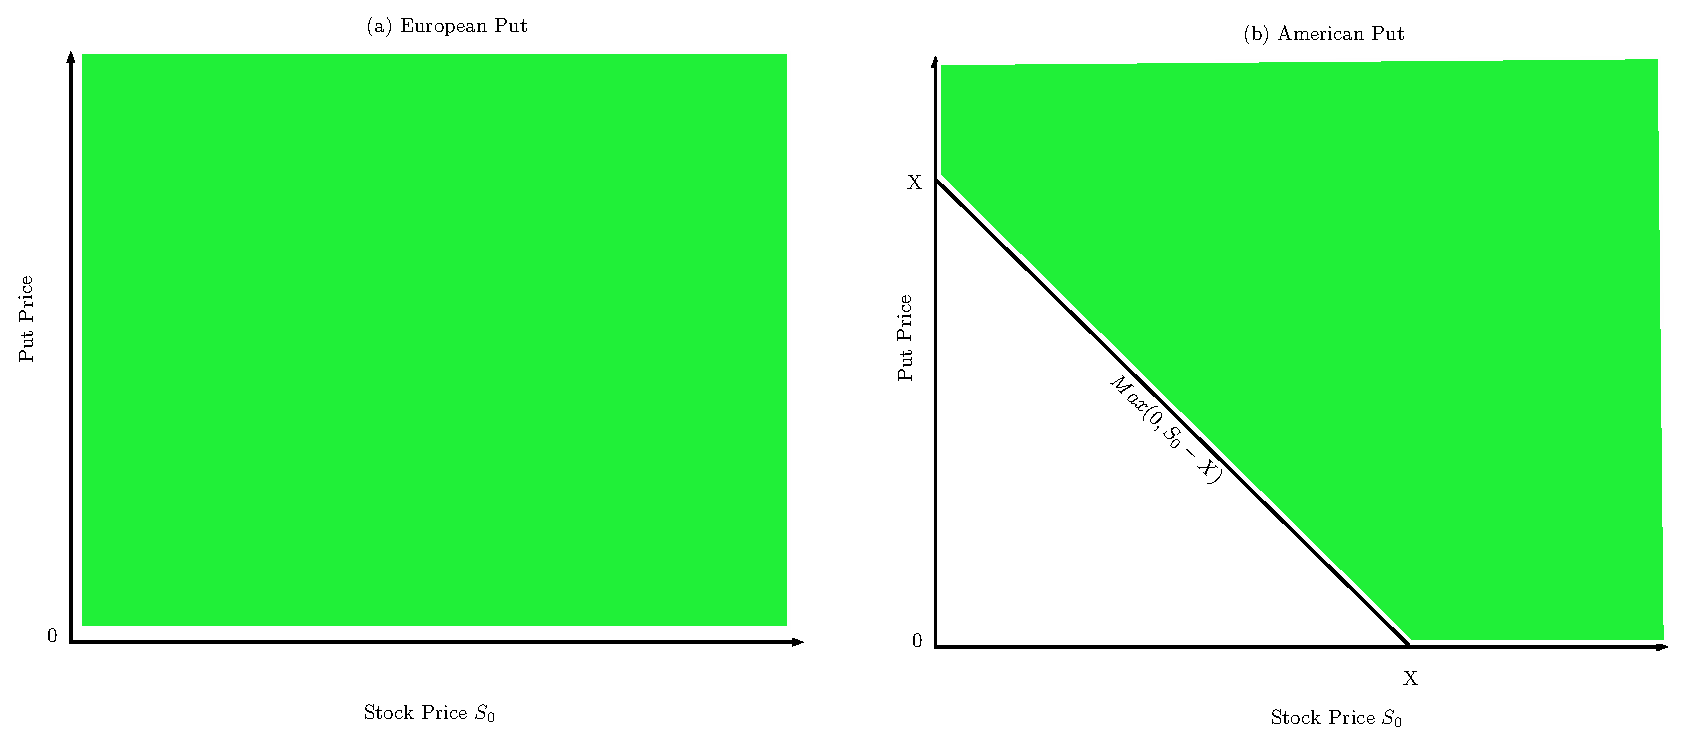
\includegraphics[scale=0.45]{images/fig:PutMin.eps}
                    \caption{Minimum Value of European \& American Puts}
                    \label{fig:PutMin}                
                \end{figure}
                
            Figure \ref{fig:PutMin} illustrates these points for puts. The European put price lies somewhere in the shaded are of Figure \ref{fig:PutMin} (a). The American put price lies somewhere in the shaded are of Figure \ref{fig:PutMin} (b).
            
        \begin{tcolorbox}[colback=blue!5!white,colframe=blue!75!black, title=Sticky Note]
            The intrinsic value of an American put is the greater of ero or the difference bwteen the exercise price and the stock price 
        \end{tcolorbox} 
           
            The value, $Max(0, X -S_0$ is call the put's \textit{intrinsic value}. An in-the-money put has a postive intrinsic value, whiel an out-of-the-money put has no intrinsic value. The difference netween the put price and the intrisic value is the \textit{time value} or \textit{speculative value}
            
            The time value is defined as $P_a(S_0,T,X) - Max(0, X - S_0)$. As with calls, the time value reflects what an investor is willing to pay for the uncertainty of the final outcome. 
         
                \begin{table}[h]
                    \centering
                    \caption{Intrinsic Value and Time Values of DCRB Puts}
                    \label{tab:PutTime}
                    \begin{tabular}[h]{L{1.5cm} L{1.5cm} | L{1cm} L{1cm} | L{1cm} L{1cm} | L{1cm} L{1cm} }
                    \toprule
                        \multicolumn{2}{c}{} & \multicolumn{2}{c}{May} & \multicolumn{2}{c}{June} & \multicolumn{2}{c}{July} \\\cline{3-8}
                        Exercise Price & Intrinsic Value  & Time Value & Put Price & Time Value & Put Price & Time Value & Put Price \\
                    \midrule
                        120.00 & 0.00 & 2.75 & 2.75 & 9.25 & 9.25 & 13.65 & 13.65 \\
                        125.00 & 0.00 & 4.60 & 4.60 & 11.50 & 11.50 & 16.60 & 16.60 \\    
                        130.00 & 4.06 & 3.29 & 7.35 & 11.19 & 14.25 & 15.59 & 19.65 \\
                    \bottomrule
                    \end{tabular}
                \end{table}    
    
            Table \ref{tab:PutTime} presents the intrinsic value and time values of DCRB puts. Note how the values increase with time to expiration. 
            
        \begin{tcolorbox}[colback=blue!5!white,colframe=blue!75!black, title=Sticky Note]
            The time value of an American put is the difference between the put price and the intrinsic value. 
        \end{tcolorbox}            
            
            The intrinsic value specification, $Max(0, X - S_0)$ does not hold for European puts. This is because the option must be exercisable for an investor to execute the arbitrage transaction previously described. European Puts can indeed sell for less than the intrisic value. 
            
        \subsubsection{Maximum Value of a Put}
            At expiration, the payoff from a European put is the $Max(X - S_T)$. The best outcome that a put holder can expect is for the company to go bankrupt. In that case, the stock will be worthless and the put holder will be able to sell the shares to the put writer for $X$ dollars. Thus, the present value of the exercise price is the European put is the european put's maximum possible value 
                \begin{equation}
                    P_e(S_0, T, X) \leqq X(1+r)^{-T}
                \end{equation}
            Since an American put can be exercised at any time, its maximum value is the exercise price: 
                
                \begin{equation}
                    P_a(S_0,T,X) \leqq X
                \end{equation}
                
            
        \begin{tcolorbox}[colback=blue!5!white,colframe=blue!75!black, title=Sticky Note]
            The maximum value of an European Put is the present value of the exercise price. The maximum value of an American put is the exercise price. 
        \end{tcolorbox}             
            
            Figure \ref{fig:PutMinMax} adds the maximum value rule to Figure \ref{fig:PutMin}. Although the range of possible values is reduced somewhat, there is still a broad range of possible values. 
            
                \begin{figure}[h]
                    \centering
                        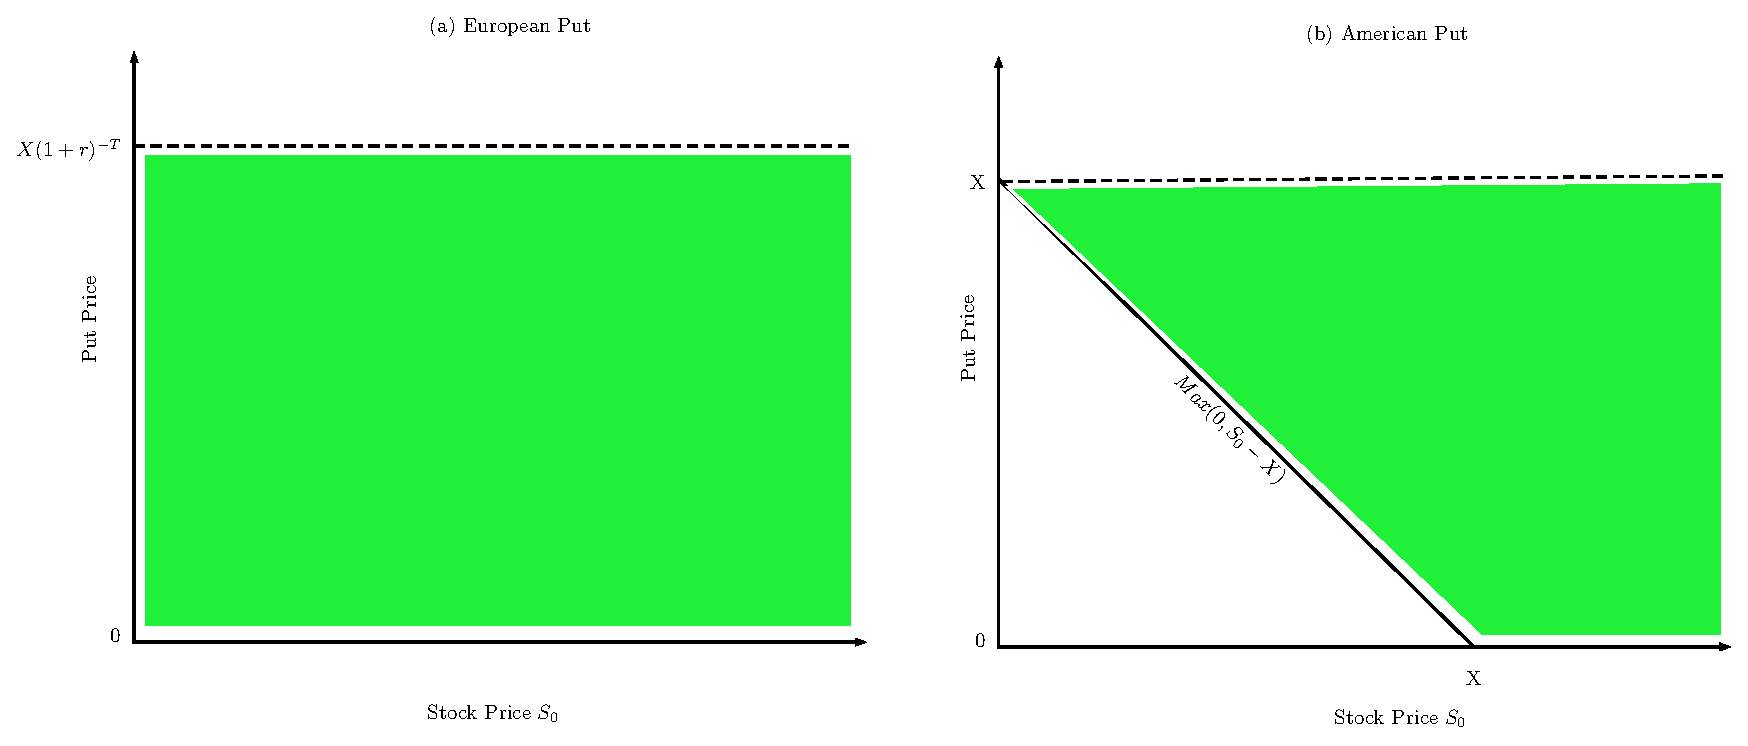
\includegraphics[scale=0.45]{images/fig:PutMinMax.eps}
                    \caption{Minimum \& Maximum Values of European \& American Puts}
                    \label{fig:PutMinMax}                
                \end{figure}            
                
        \subsubsection{Value of a Put at Expiration}
            On the put's expiration date, no time value will remain. Expiring American puts therefore are the same as European puts. The value of either types of put must be the intrinsic value. Thus,
            
                \begin{equation}
                    P(S_T, 0, X) = Max(0, X - S_T)
                \end{equation}
                
        \begin{tcolorbox}[colback=blue!5!white,colframe=blue!75!black, title=Sticky Note]
            At expiration, a put option is worth the intrinsic value 
        \end{tcolorbox}               
            
            If $X > S_T$ and put price is less than $X - S_T$, investors can buy the put and and stock, and exercise the put for an immediate riskfree profit. If the put expires out-of-the-money $X < S_T$, it will be worthless. 

                \begin{figure}[h]
                    \centering
                        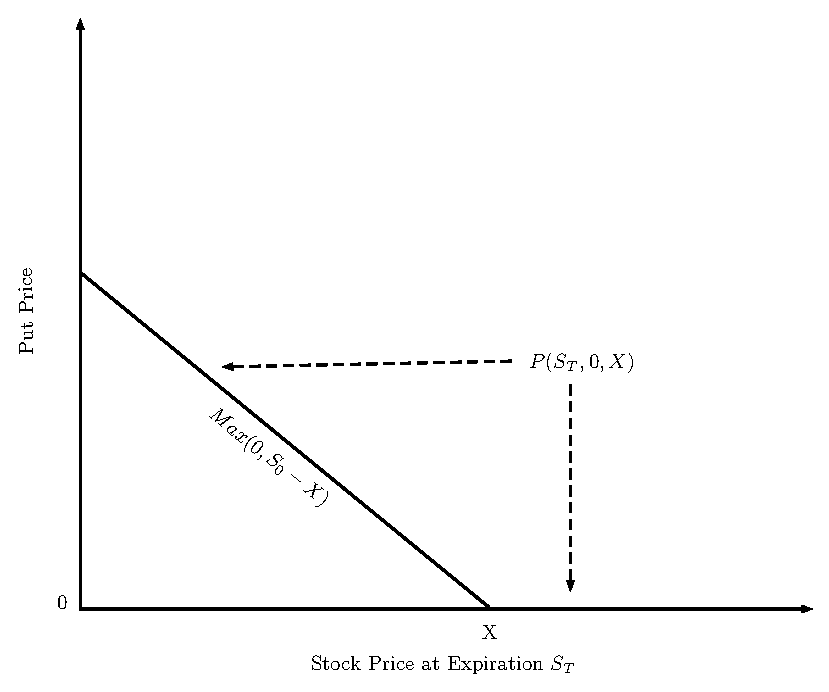
\includegraphics[scale=0.45]{images/fig:PutExp.eps}
                    \caption{Minimum \& The Value of a Put at Expiration}
                    \label{fig:PutExp   }                
                \end{figure} 
            
            Figure \ref{fig:PutExp} illustrates the value of the put at expiration.
            
        \subsubsection{Effect of Time to Expiration}
        
            Consider two American puts, one with a time to expiration of $T_1$ and the other with a time to expiration of $T_2$, where $T_2 > T_1$. Now, assume today is the expiration date of the shorter-lived put. The stock price is $S_{t_1}$. The expiring put is worth $Max (0, X - S_{T_1})$. The other put, which has a remaining time to expiration of $T_2 - T_1$, is worth at least $Max(0, X - S_{t_1})$. Consequently, it must be true at time $0$, we must have, 
                \begin{equation}
                    P_a(S_0, T_2, X) \geqq P_a (S_0, T_1, X)
                \end{equation}
                
        \begin{tcolorbox}[colback=blue!5!white,colframe=blue!75!black, title=Sticky Note]
            A longer-lived American put must always be worth at least as much as a shorter-lived American put with the same terms 
        \end{tcolorbox}                  
                
            Note that the two puts could be worth the same; however, this would occur only if both puts were very deeply-in or deeply-out of the money. Even then, the longer-livef put would likely be worth a little more than the shorter-lived put. The longer-lived put can do everything the shorter-lived put can do and has an additional period of time in which to increase in value. 
                
            The prinicples that underlie the time value of a put are the same as those that underlie the time value of a call. The time value is the largest when the stock price is near the exercise price and smallest when the stock price is very high or very low relative to the exercise price. With these points in mind, we can now see that the American put price looks live Figure (\ref{fig:APutExp}. As expiration approaches, the put price curve approaches the intrinsic value, which is due to the time value decay. At expiration the put price equals the intrinsic value, as in Figure \ref{fig:APutExp}. 

                \begin{figure}[h]
                    \centering
                        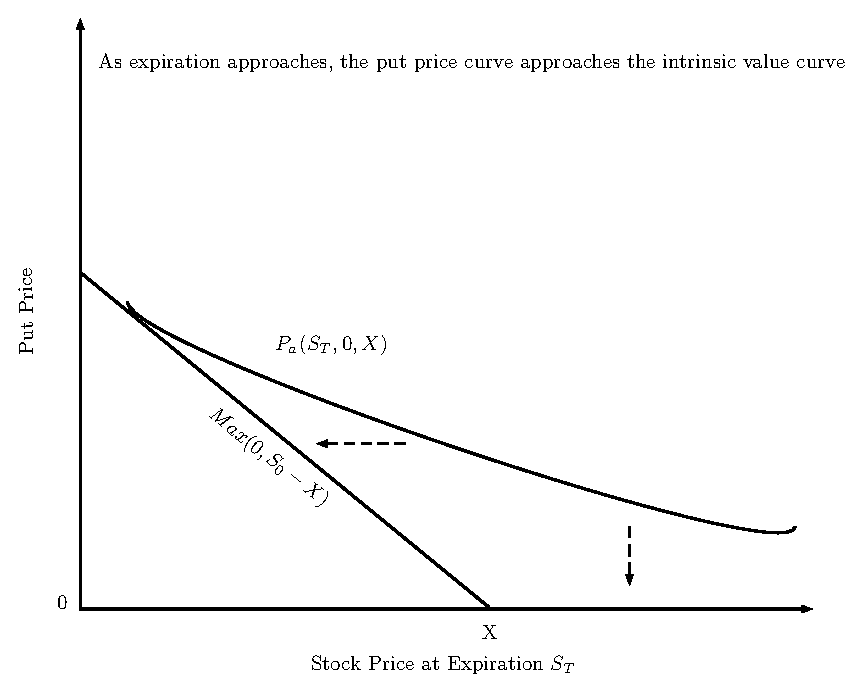
\includegraphics[scale=0.45]{images/fig:APutExp.eps}
                    \caption{The Price curve for American Puts}
                    \label{fig:APutExp}                
                \end{figure}
            
            The relationship between time to expiration and put price is more complex for European puts. Think of buying a put as deferring the sale of stock at the exercise price, $X$. The further into the future the expiration date, the longer the put holder must wait sell to sell the stock and receive X dollars. This can make the longer-lived European put less valiuable than the shorter-lived one. This does not hold for American puts, becuase the holder can always exercise it and receive $X$ dollars today. 
            ,km m
            For a European put, the longer time tp expiration is both an advantage - the greater time value - the long wait time to receive the exercise price. The time value effect tends to dominate, however, and in most cases longer-lived puts will be more valuable than shorter-lived puts. Because DCRB puts are American options, the longer-term put should be expected to show higher prices. A check of their premiums, shown in Table, confirms this point.
        
        \subsubsection{Effect of Exercise Price}
            
            \begin{definition}{\textbf{The Effect on Option Value}}
                
                Consider two European puts identical in all respectss except exercise price. One put has an exercise price of $X_1$ and a premium of $P_e(S_0, T, X_1)$; the other has an exercise price of $X_2$ and a premium of $P_e(S_0, T, X_2)$. As before $X_2 > X_1$. Which put option will be more valuable?
                
        \begin{tcolorbox}[colback=blue!5!white,colframe=blue!75!black, title=Sticky Note]
            The price of a European put must b at least as high as the price of an otherwise identical European put with a lower exerise price.
        \end{tcolorbox} 
                
                Consider the two portfolios. Portfolio A consists of a long position in the put priced at $P_e(S_0, T, X_2$ and a short position in the put priced at $P_e(S_0, T, X_1)$. Portfolio B consists of a long position in risk-free bonds with a face value $X_2 - X_1$ and a present value of $(X_2 - X_1)(1 + r)^{-T}$. Table \ref{tab:PutPayoff} presents these portfolios payoff at expiration. 

                \begin{table}[h]
                    \centering
                    \caption{The Effect of Exercise Price on Put Value: Payoffs at Expiration of Portfolio A \&  B}
                    \label{tab:PutPayoff}
                        \begin{tabular}{llccc}
                             \toprule
                                & &\multicolumn{3}{c}{Payoffs from Portfolio Given Stock Price at Expiration} \\
                             Portfolio & Current Value & $S_T < X_1$ & $X_1 \leqq S_T < X_2$ & $X_1 < X_2 \leqq S_T$ \\\hline
                                \multirow{3}*{A} & $-P_e(S_0,T,X_1)$ & $-X_1 + S_T$ & $0$ & $0$ \\
                                & $+P_e(S_0,T,X_2)$ & \underline{$X_2 - S_T$} & \underline{$X_2 - S_T$} & \underline{$0$} \\
                                & & \emph{$x_2 - x_1 > 0$} & \emph{$x_2 - x_1 > 0$} & $0$ \\\midrule
                                B & $(x_2 - x_1)(1 + r)^{-T}$ & $x_2 - x_1 > 0$ & $x_2 - x_1 > 0$ & $x_2 - x_1 > 0$ \\\bottomrule                  
                        \end{tabular}
                \end{table}                 

                For portfolio A, all outcomes are nonnegative. Because this portfolio cannot produce a cash outflow for the holder, the price of the put purchased must be no less than the price of the put sold; that is 
                
                    \begin{equation}
                        P_e(S_0,T,X_2) \geqq P_e(S_0,T,X_1)
                    \end{equation} 
                    
                To understand why this is so, consider what would happen if it were not. Suppose that the price of the put sold were greater than the price of the put purchased. Then, an investor would receive more for the put sold than would be paid for the put purchased. That would produce a net positive cash flow up front, and, from Table \ref{tab:PutPayoff}, there would be no possibility of having to pay out any cash at expiration. This would be like a loan you don't have to payback. 
                    
                The intuition behind  why a put with a higer a higher exercise price is worth more than one with a lowwer exercise price is quite simple. A put is an option to sell stock at a fixed price. The higher the price at which the put holder  can sell the stock, the more attractive the put. 
                
        \begin{tcolorbox}[colback=blue!5!white,colframe=blue!75!black, title=Sticky Note]
            The price of an American put must be at least as high as the price of an otherwise identical American put with a lower exercise price.
        \end{tcolorbox}            
                
                Suppose that they were American puts. In that case, the put with the lower exercise price could be exercised early. For example, let the stock price at time $t$ prior to expiration be $S_t$, where $S_t < X_1$. Let the option with exerise price $X_1$ be exercised. Then the investor simply exercise the option with the exerise price $X_2$. The cash flow from these two transactions is $$-(X_1 - S_t)+(X_2 - S_t) = X_2 - X_1$$ which is positive. Early exercise will not generate a negative cash flow. Thus, our result holds for American puts as well A European puts.
            \end{definition}
            
            \begin{definition}{\textbf{Limits on the Difference in Premiums}}
            
                Now let us consider the outcomes of portfolio A and B. We see that portfolio B's outcome are never less than portfolio A's. Therefore, no one would pay more for portfolio A than for portfolio B. That is
                    \begin{equation}
                        (X_2 - X_1)(1 + r)^{-T} \geqq P_e(S_0,T,X_2) - P_e(S_0,T,X_1)
                    \end{equation}
                This result does not, however, hold for American  puts. If the puts were American and both were exercised, the investor would receive $X_2 - X_1$ dollars. This amounnt would be invested in risk-free bonds and would earn invesr over the option's remaining lives. At expiration, the inbestor would have more than $X_2 - X_1$, the payoff from portfolio B.
                
                Since the difference in exercise prices is greater than the present value of the difference in exercise prices, we can state that for European puts, 
                    \begin{equation}
                        (X_2  - X_1 ) \geqq P_e(S_0,T,X_2) - P_e(S_0, T, X_1)
                    \end{equation}
                This mean that the difference in puts premiums cannot exceed the difference in exercise fprices. This result holds for American as well as European puts. To see this, let portfolio B's bonds have a face value of $(X_2 - X_1)(1 + r)^T$ and a present value of $(X_2 - X_1)$. If early exercise occurred at time $t$, the most the holder of portfolio A would have at expiration is $$(X_2 - X_1)(1 + r)^{T- t}$$ The holder of portfolio B would have a larger amount, $(X_2 - X_1)(1 + r)^T$. So again portfolio A would never pay more at expiration than portfolio B. Therefore, the current value of portfolio A, $P_a(S_0,T,X_2) - P_a(S_0,T,X_1)$, could not exceed the current value of portfolio B, $X_2 - X_1$. 
                
        \begin{tcolorbox}[colback=blue!5!white,colframe=blue!75!black, title=Sticky Note]
            The difference in the prices of two American puts that differ only by exercise price cannot exceed the difference in their exercise prices.
        \end{tcolorbox}                  
                
                Thus, 
                    \begin{equation}
                        X_2 - X_1 \geqq P_a(S_0, T, X_2) - P_a(S_0, T, X_1)
                    \end{equation}
                    
                Table \ref{tab:PutExPrice} \footnotemark shows the difference between the put premiums and exercise price for the DCRB puts. Since these are American puts, we would expect only the difference in ther put premiums will not exceed the present values of the diffrence in their exercise prices - which indeed is the case. In addition, the difference in premiums do not exceed the present values of the difference in exercise prices. 
                
                \footnotetext{ Note: we use Table \ref{tab:DCRBRiskTime} to calculate the present value of the exercise price spreads. For example, the present value of the May 120, 125 Put spread is $$PV_{120, 125} = 5(1 + \frac{4.57}{100})^-0.0192$$ }
                
                \begin{table}[h]
                    \centering
                    \caption{The Relationship between Exercise Price \& Put Price for DCRB Puts}
                    \label{tab:PutExPrice}
                    \begin{tabular}[h]{L{1.5cm} L{1.5cm} | L{1cm} L{1cm} | L{1cm} L{1cm} | L{1cm} L{1cm} }
                    \toprule
                        \multicolumn{2}{c}{} & \multicolumn{2}{c}{May} & \multicolumn{2}{c}{June} & \multicolumn{2}{c}{July} \\\cline{3-8}
                        Exercise Price & Spread Future Value & Spread Present Value & Put Spread & Spread Present Value & Put Spreadd & Spread Present Value & Put Spread \\
                     \midrule
                        120, 125 & 5    & 4.9957    & 1.85  & 4.9787    & 2.25  & 4.9611    & 2.95 \\
                        120, 130 & 10   & 9.9914    & 4.60  & 9.9573    & 5.00  & 9.9222    & 6.00 \\
                        125, 130 & 5    & 4.9957    & 2.75  & 4.9787    & 2.75  & 4.9611    & 3.05 \\
                    \bottomrule
                    \end{tabular}
                \end{table}                  
                
            \end{definition}
            
        \subsubsection{Lower Bound of a European Put}
        
            The fact that the minimum value of an American put is $Max(), X - S_0)$, does not hold for a European put because it cannot be exercised early. However, it is possible to derive the lower bound of an European put. 
            
            Consider two portfolios A and B. Portolifo A consisting of a single share of stock. Portfolio B consists of a short position in a European put priced at $P_e(S_0,T,X)$ and a long position in risk-free bonds with a face value of $X$ and a present value of $X(1+r)^{-T}$. The payoffs at expiration from these portfolios are shown in Table \ref{tab:EuroPutLB}. 
            
                \begin{table}[h]
                    \centering
                    \caption{Lower Bound of a European Put: Payoffs at Expiration of Profilios A \& B}
                    \label{tab:EuroPutLB}
                    \begin{tabular}[h]{L{1cm} L{5cm} L{5cm} L{3cm}}
                    \toprule
                        \multicolumn{2}{c}{} & \multicolumn{2}{c}{Payoffs from Portfolio Given Stock Price at Expiration} \\\cline{3-4}
                        Portfolio & Current Value & $S_T < X$ & $S_T \geqq X$ \\
                     \midrule
                        A   & $S_0$                             & $S_T$                 & $S_T$ \\
                        B   & $X(1+6r)^{-T} - P_e(S_0, T, X)$   & $X - (X - S_T) = S_T$ & $X$ \\
                    \bottomrule
                    \end{tabular}
                \end{table}             
                
            Portfolio A's outcome is always at leasst as favorable as portfolio B's. Therefore, no one would be willing to pay more for portfolio B than portfolio A. Portfolio A's current value must be less than portfolio B's; that is, 
                \begin{equation}
                    S_0 \geqq X(1+r)^{-T} - P_e(S_0, T, X)
                \end{equation}
                
            Rearranging this statement gives
            
                \begin{equation}
                    P_e(S_0,T,X) \geqq X(1 + r)^{-T} - S_0
                \end{equation}
                
            If the present value of the exercise price is less than the stock price, this lower bound will be negative. Since we know that a put cannot be worth less than  zero, we can say that
            
                \begin{equation}
                    P_e(S_0,T,X) \geqq Max \left[ 0, X(1+r)^{-T} - S_0 \right]
                \end{equation}

                \begin{figure}[h]
                    \centering
                        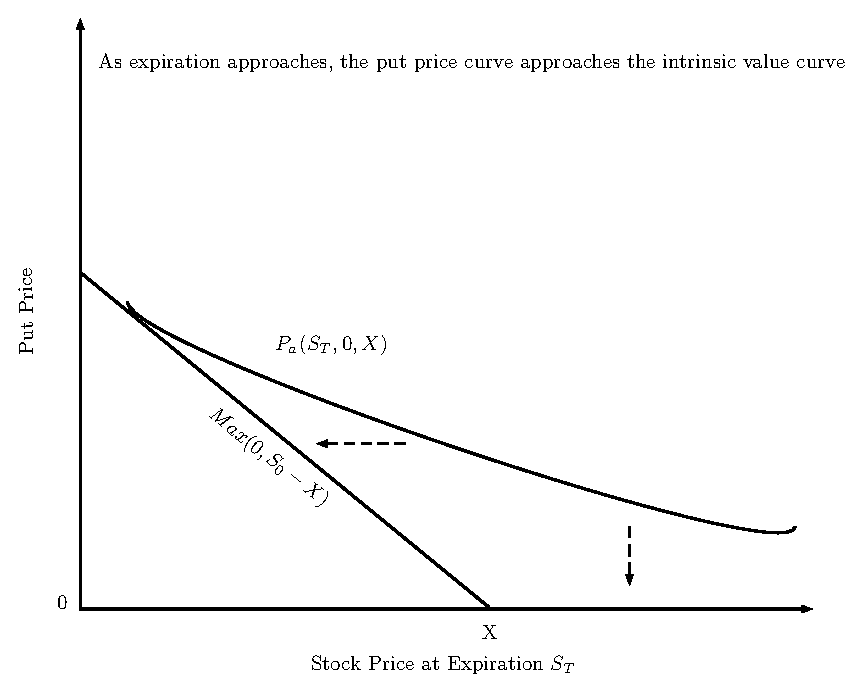
\includegraphics[scale=0.45]{images/fig:APutExp.eps}
                    \caption{The Price curve for American Puts}
                    \label{fig:APutExp}                
                \end{figure}
                
            
        \subsubsection{American Put vs. European Put}
        \subsubsection{Early Exerise of American Puts}
        \subsubsection{Put-Call Parity}
        \subsubsection{Effect of Interest Rates}
        \subsubsection{Effect of Stock Volatility}
        
\section{Options Pricing Models: The Binomial Model}

\section{Options Pricing Models: The Black-Scholes-Merton Model}

\section{Basic Options Strategies}

\section{Advanced Options Strategies}
    
    
\newpage
\chapter{FORWARDS, FUTURES AND SWAPS}
\section{Structure of Forwards and Futures Market}
\section{Principles of Pricing Forwards, Futures and Option Market}
\section{Forwads and Futures Hedging, Spreads and Other Strategies}
\section{Swaps}

\newpage
\chapter{OPTIONS PRICING THEORY: I}
\section{Put-Call Parity and Other Options Relationships}
\section{Binomial Options Pricing: Basic Concepts}
\section{Binomial Options Pricing: Selected Topics}
\section{Black-Scholes Formula}
\section{Market Making and Delta Hedging}
\section{Exotic Options: 1}

\newpage
\chapter{FINANCIAL ENGINEERING AND APPLICATIONS}
\section{Financial Engineering and Security Design}
\section{Corporate Applications}
\section{Real Options}

\newpage
\chapter{OPTIONS PRICING THEORY: II}
\section{Lognormal Distribution}
\section{Monte Carlo Valuation}
\section{Brownian Motion and Ito Lemma}
\section{Black-Scholes Equation}
\section{Risk Neutral and Martingale Pricing}
\section{Exotic Options: II}
\section{Volatility}
\section{Interest Rates and Bond Derivatives}
\section{Value Added Risk}
\section{Credit Risk}



\newpage
\chapter{Bibiography}
\printbibliography




\end{document}